\documentclass{beamer}

\begin{document}
	
	\begin{frame}
	\frametitle{Vision: Seeing an Image}
		\begin{itemize}
			\item When the human vision sees things, it sees a picture, an image. But what does the computer see?
			
			\begin{figure}
				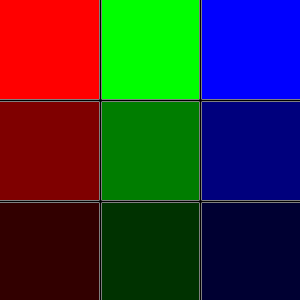
\includegraphics[scale = 0.5]{colors}
				\caption{3 pixel by 3 pixel grid}
			\end{figure}
		\end{itemize}
	\end{frame}
	
	
	
	
	\begin{frame}
	\frametitle{Image as a Matrix}
		\begin{itemize}
			\item As it turns out, the computer sees an image as a matrix of pixels:
		
			\item \[
			\left( \begin{array}{ccc}
			P_{1} & P_{2} & P_{3} \\
			P_{4} & P_{5} & P_{6} \\
			P_{7} & P_{8} & P_{9}
			\end{array} \right)
			\]
		
			\item With $P_{i}$ = (\colorbox{blue}{B},\colorbox{green}{G},\colorbox{red}{R})
		
			\item While different compositions of \colorbox{blue}{B}\colorbox{green}{G}\colorbox{red}{R}values make up unique colors (each color component ranges from 0 to 255).
		\end{itemize}
	\end{frame}
	
	
	\begin{frame}
	\frametitle{Computer Vision}
		\begin{itemize}
			\item So the following image has two forms.
			
			\item Its image form 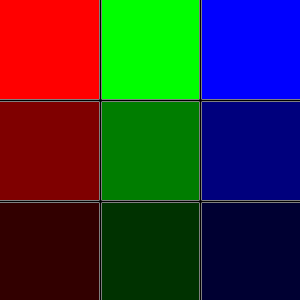
\includegraphics[scale = 0.4]{colors}
			
			\item And its matrix form
						\[
						\left( \begin{array}{lll}
						(\colorbox{blue}{0},\colorbox{green}{0},\colorbox{red}{255}) & (\colorbox{blue}{0},\colorbox{green}{255},\colorbox{red}{0}) & (\colorbox{blue}{255},\colorbox{green}{0},\colorbox{red}{0}) \\
						(\colorbox{blue}{0},\colorbox{green}{0},\colorbox{red}{125}) & (\colorbox{blue}{0},\colorbox{green}{125},\colorbox{red}{0}) & (\colorbox{blue}{125},\colorbox{green}{0},\colorbox{red}{0}) \\
						(\colorbox{blue}{0},\colorbox{green}{0},\colorbox{red}{50}) & (\colorbox{blue}{0},\colorbox{green}{50},\colorbox{red}{0}) & (\colorbox{blue}{50},\colorbox{green}{0},\colorbox{red}{0})
						\end{array} \right)
						\]
		\end{itemize}
	\end{frame}
	
	
	\begin{frame}
	\frametitle{Computer Vision: Videos}
		\begin{itemize}
			\item A video is a sequence of images.
			
			\pause
			
			\item And because images are also matrices, a video can also be a sequence of matrices.
			
			\pause
			
			\item Now that we have a sequence of matrices, what can we do?
			
			\pause
			
			\item \large SCENE CHANGES!
		\end{itemize}
	\end{frame}
	
	
	\begin{frame}
	\frametitle{Computer Vision: Scene Changes}
	
		\begin{itemize}
			\item A scene change is a change in scene!
			
			\item 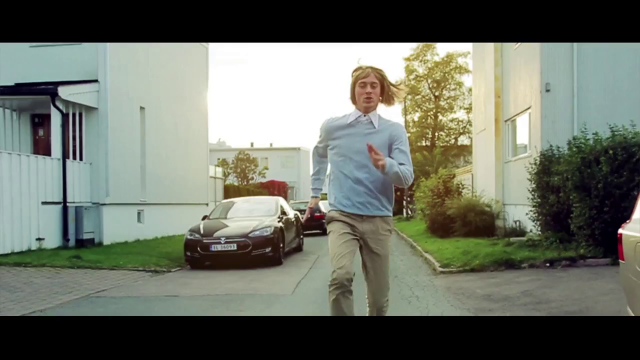
\includegraphics[scale = 0.23]{runningFrame3375} ~~~~ 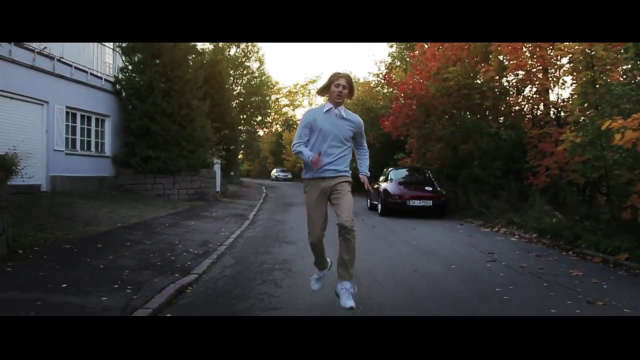
\includegraphics[scale = 0.23]{runningFrame3400}
			
			\pause
			
			\item How does a computer see this scene change?
			
			\pause 
			
			\item What in the sequence of matrices indicates this scene change?
		\end{itemize}
		
		
	\end{frame}
\end{document}

